% Slide: Curve Representation Comparison
\begin{frame}{Curve Representations in Geometry}
  Comparing representations of a geometric curve $\vect{C}$:
  \begin{columns}[T]
    \begin{column}{0.31\textwidth}
      \begin{block}{Explicit}
        \centering
        \scalebox{0.8}{
          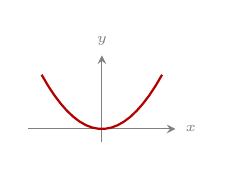
\begin{tikzpicture}[scale=0.85, >=stealth]
            \draw[->, gray, thin] (-1.1,0) -- (1.1,0) node[right, font=\tiny] {$x$};
            \draw[->, gray, thin] (0,-0.2) -- (0,1.1) node[above, font=\tiny] {$y$};
            \draw[thick, red!70!black, domain=-0.9:0.9, samples=20] plot (\x, {\x*\x});
          \end{tikzpicture}
        }
        \par\vspace{0.1cm}
        \centering\small \textcolor{red!70!black}{$y = x^2$}
        \par\vspace{0.15cm}
        \raggedright\scriptsize
        Easy to compute, but cannot represent vertical lines or multiple-valued curves (e.g., circles).
      \end{block}
    \end{column}
    \begin{column}{0.31\textwidth}
      \begin{block}{Implicit}
        \centering
        \scalebox{0.8}{
          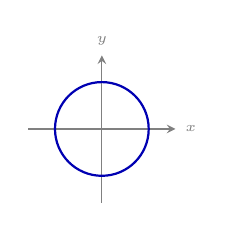
\begin{tikzpicture}[scale=0.85, >=stealth]
            \draw[->, gray, thin] (-1.1,0) -- (1.1,0) node[right, font=\tiny] {$x$};
            \draw[->, gray, thin] (0,-1.1) -- (0,1.1) node[above, font=\tiny] {$y$};
            \draw[thick, blue!70!black] (0,0) circle (0.7);
          \end{tikzpicture}
        }
        \par\vspace{0.1cm}
        \centering\small \textcolor{blue!70!black}{$x^2 + y^2 - R^2 = 0$}
        \par\vspace{0.15cm}
        \raggedright\scriptsize
        Can represent arbitrary shapes/topologies, but hard to parameterize or evaluate coordinates directly.
      \end{block}
    \end{column}
    \begin{column}{0.34\textwidth}
      \begin{alertblock}{Parametric}
        \centering
        \scalebox{0.8}{
          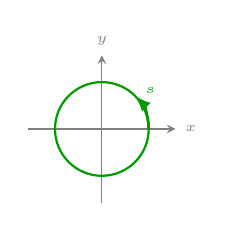
\begin{tikzpicture}[scale=0.85, >=stealth]
            \draw[->, gray, thin] (-1.1,0) -- (1.1,0) node[right, font=\tiny] {$x$};
            \draw[->, gray, thin] (0,-1.1) -- (0,1.1) node[above, font=\tiny] {$y$};
            \draw[thick, green!60!black] (0,0) circle (0.7);
            \draw[green!60!black, ->, >=latex, line width=1pt] (0.7,0) arc (0:45:0.7) node[right, font=\tiny, yshift=2pt] {$s$};
          \end{tikzpicture}
        }
        \par\vspace{0.1cm}
        \centering\small \textcolor{green!60!black}{$\begin{cases} x(s) = R\cos(s) \\ y(s) = R\sin(s) \end{cases}$}
        \par\vspace{0.15cm}
        \raggedright\scriptsize
        \textbf{Standard in CAD}. Easy to generate coordinates, trace boundaries, and map variables. Flexible dimension scaling.
      \end{alertblock}
    \end{column}
  \end{columns}
\end{frame}

% Slide: Why IGA?
\begin{frame}{Why IGA?}
  \small
  Isogeometric Analysis unifies geometry and numerical simulation:

  \vspace{0.3cm}
  \begin{columns}[T]
    \begin{column}{0.31\textwidth}
      \begin{block}{CAD Splines}
        \footnotesize
        Adopts native spline basis functions used in CAD, eliminating separate meshing steps.
      \end{block}
    \end{column}

    \begin{column}{0.31\textwidth}
      \begin{block}{Exact Geometry}
        \footnotesize
        Preserves true curved boundaries (arcs, fillets) without geometric approximation errors.
      \end{block}
    \end{column}

    \begin{column}{0.31\textwidth}
      \begin{block}{High Regularity}
        \footnotesize
        Inter-element $C^{p-1}$ continuity yields smooth stress fields and higher accuracy per DOF.
      \end{block}
    \end{column}
  \end{columns}
\end{frame}

% Slide: Core Ingredients of IGA
\begin{frame}{The Core Ingredients of IGA}
  \begin{columns}[T]
    \begin{column}{0.48\textwidth}
      \begin{block}{1. Knot Vector}
        \scriptsize
        Ordered set of parametric coordinates:
        \[
          \Xi = \{\xi_0, \xi_1, \dots, \xi_m\}
        \]
        Non-zero knot spans partition the domain into elements.
      \end{block}
      \vspace{0.1cm}
      \begin{block}{3. Weights (NURBS)}
        \scriptsize
        Weights $w_i$ rationalise the basis functions:
        \[
          R_{i,p}(\xi) = \frac{N_{i,p}(\xi)w_i}{\sum_j N_{j,p}(\xi)w_j}
        \]
        Allows exact representation of conic shapes.
      \end{block}
    \end{column}

    \begin{column}{0.48\textwidth}
      \begin{block}{2. B-Spline Basis}
        \scriptsize
        Polynomial basis constructed via Cox-de Boor:
        \[
          N_{i,p}(\xi) = \tfrac{\xi-\xi_i}{\xi_{i+p}-\xi_i}N_{i,p-1} + \tfrac{\xi_{i+p+1}-\xi}{\xi_{i+p+1}-\xi_{i+1}}N_{i+1,p-1}
        \]
        Yields $C^{p-1}$ continuity across internal elements.
      \end{block}
      \vspace{0.1cm}
      \begin{block}{4. Control Points}
        \scriptsize
        Physical coordinates $\vect{P}_i$ that parameterize geometry:
        \[
          \vect{C}(\xi) = \sum_i R_{i,p}(\xi)\,\vect{P}_i
        \]
        Read directly from CAD formats (\textbf{`.stp`}, \textbf{`.igs`}).
      \end{block}
    \end{column}
  \end{columns}
\end{frame}

% Slide: B-Spline Basis Functions — figure copied from thesis Ch.3
\begin{frame}{B-Spline Basis Functions}
  \begin{columns}[T]
    \begin{column}{0.50\textwidth}
      Over open knot vector $\Xi=\{\xi_0,\ldots,\xi_m\}$, the \textbf{Cox-de Boor recurrence}:
      \[
        N_{i,0}(\xi) = \begin{cases}1 & \xi_i\le\xi<\xi_{i+1}\\0&\text{otherwise}\end{cases}
      \]
      \[
        N_{i,p}(\xi) = \tfrac{\xi-\xi_i}{\xi_{i+p}-\xi_i}N_{i,p-1} + \tfrac{\xi_{i+p+1}-\xi}{\xi_{i+p+1}-\xi_{i+1}}N_{i+1,p-1}
      \]
      \par\vspace{0.2cm}
      \textbf{Key Properties:}
      \begin{itemize}
        \scriptsize
        \item \textbf{Partition of Unity:} $\sum_{i} N_{i,p}(\xi) = 1 \quad \forall\,\xi$
        \item \textbf{Non-negativity:} $N_{i,p}(\xi) \ge 0 \quad \forall\,\xi, i$
        \item \textbf{Local Support:} $N_{i,p}(\xi) = 0$ outside $[\xi_i, \xi_{i+p+1})$
      \end{itemize}
    \end{column}
    \begin{column}{0.48\textwidth}
      \centering
      % B-spline plot — copied from thesis Fig 3.1
      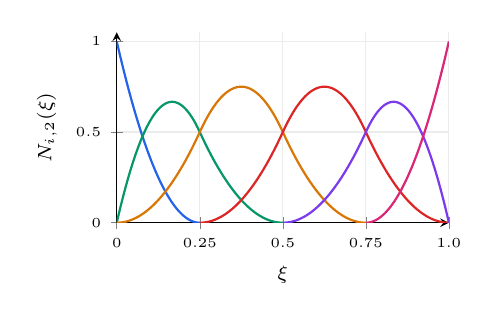
\begin{tikzpicture}[scale=1.0, >=stealth]
        \definecolor{n0color}{RGB}{37,99,235}
        \definecolor{n1color}{RGB}{5,150,105}
        \definecolor{n2color}{RGB}{217,119,6}
        \definecolor{n3color}{RGB}{220,38,38}
        \definecolor{n4color}{RGB}{124,58,237}
        \definecolor{n5color}{RGB}{219,39,119}
        \begin{axis}[
            width=5.8cm, height=4.0cm,
            xmin=0, xmax=1, ymin=0, ymax=1.05,
            xlabel={$\xi$}, ylabel={$N_{i,2}(\xi)$},
            tick label style={font=\tiny},
            xlabel style={font=\scriptsize},
            ylabel style={font=\scriptsize},
            xtick={0,0.25,0.5,0.75,1.0},
            xticklabels={0, 0.25, 0.5, 0.75, 1.0},
            grid=both, grid style={gray!15},
            axis lines=left
          ]
          % N_{0,2}
          \addplot[n0color, thick, domain=0:0.25, samples=50] {(1-4*x)^2};
          % N_{1,2}
          \addplot[n1color, thick, domain=0:0.25, samples=50] {8*x-24*x^2};
          \addplot[n1color, thick, domain=0.25:0.5, samples=50] {8*(0.5-x)^2};
          % N_{2,2}
          \addplot[n2color, thick, domain=0:0.25, samples=50] {8*x^2};
          \addplot[n2color, thick, domain=0.25:0.5, samples=50] {12*x-16*x^2-1.5};
          \addplot[n2color, thick, domain=0.5:0.75, samples=50] {8*(0.75-x)^2};
          % N_{3,2}
          \addplot[n3color, thick, domain=0.25:0.5, samples=50] {8*(x-0.25)^2};
          \addplot[n3color, thick, domain=0.5:0.75, samples=50] {12*(1-x)-16*(1-x)^2-1.5};
          \addplot[n3color, thick, domain=0.75:1.0, samples=50] {8*(1-x)^2};
          % N_{4,2}
          \addplot[n4color, thick, domain=0.5:0.75, samples=50] {8*(x-0.5)^2};
          \addplot[n4color, thick, domain=0.75:1.0, samples=50] {8*(1-x)-24*(1-x)^2};
          % N_{5,2}
          \addplot[n5color, thick, domain=0.75:1.0, samples=50] {(4*x-3)^2};
        \end{axis}
      \end{tikzpicture}\\[2pt]
      {\scriptsize Degree-$p=2$ basis, $\Xi=\{0,0,0,0.25,0.5,0.75,1,1,1\}$}
    \end{column}
  \end{columns}
\end{frame}

% Slide: B-Spline Curve Concept
\begin{frame}{B-Spline Curve Concept}
  \begin{columns}[T]
    \begin{column}{0.50\textwidth}
      \small
      A B-spline/NURBS curve $\vect{C}(\xi)$ is defined as:
      \[
        \vect{C}(\xi) = \sum_{i=0}^{n-1} R_{i,p}(\xi) \vect{P}_i
      \]
      \begin{itemize}
        \item $\vect{P}_i$ represent the \textbf{control points}.
        \item The control points form a piecewise linear \textbf{control polygon}.
        \item Lack of Kronecker delta property: $\vect{C}(\xi_i) \neq \vect{P}_i$ in general, except at the clamped boundary ends.
      \end{itemize}
      \par\vspace{0.2cm}
      \centering
      \href{https://cnam-internship-mumen.netlify.app/app/simulations/iga-sim/}{\beamerbutton{Interactive IGA Curve Web App}}
    \end{column}
    \begin{column}{0.48\textwidth}
      \centering
      \scalebox{0.9}{
        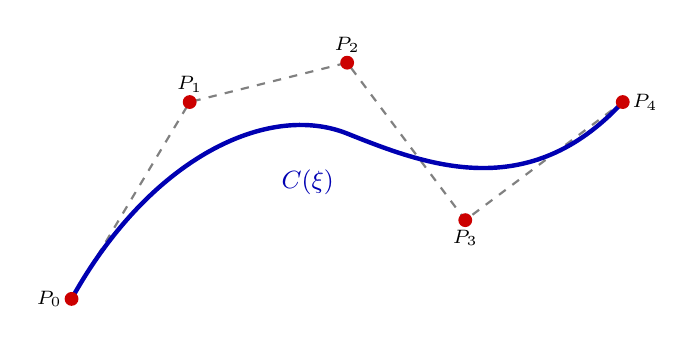
\begin{tikzpicture}[scale=1.0, >=stealth]
          \coordinate (P0) at (0, 0);
          \coordinate (P1) at (1.5, 2.5);
          \coordinate (P2) at (3.5, 3.0);
          \coordinate (P3) at (5.0, 1.0);
          \coordinate (P4) at (7.0, 2.5);

          % Draw control polygon (dashed)
          \draw[thick, gray, dashed] (P0) -- (P1) -- (P2) -- (P3) -- (P4);

          % Draw actual B-spline curve
          \draw[ultra thick, blue!70!black] (P0) .. controls (1.0,1.8) and (2.5,2.5) .. (3.5,2.1) .. controls (4.5,1.7) and (5.8,1.2) .. (P4);

          % Draw control points
          \foreach \p/\l/\pos in {P0/P_0/left, P1/P_1/above, P2/P_2/above, P3/P_3/below, P4/P_4/right} {
              \fill[red!80!black] (\p) circle (2.5pt);
              \node[\pos, font=\scriptsize] at (\p) {$\vect{\l}$};
            }
          \node[blue!70!black, above, font=\small] at (3, 1.2) {$\vect{C}(\xi)$};
        \end{tikzpicture}
      }
    \end{column}
  \end{columns}
\end{frame}

% Slide: 2D Bivariate Basis Functions
\begin{frame}{2D Bivariate Basis Functions}
  \begin{columns}[T]
    \begin{column}{0.42\textwidth}
      \small
      \textbf{Basis Function Shapes}:
      \begin{itemize}
        \item Bivariate basis shape depends on location in control net.
        \item \textbf{Boundary Basis} $R_{0,2}(\xi,\eta)$: Edge-supported, peaks at boundaries.
        \item \textbf{Internal Basis} $R_{2,2}(\xi,\eta)$: Fully internal support, peaks at center of element grid.
      \end{itemize}
    \end{column}
    \begin{column}{0.55\textwidth}
      \centering
      \scalebox{0.55}{
        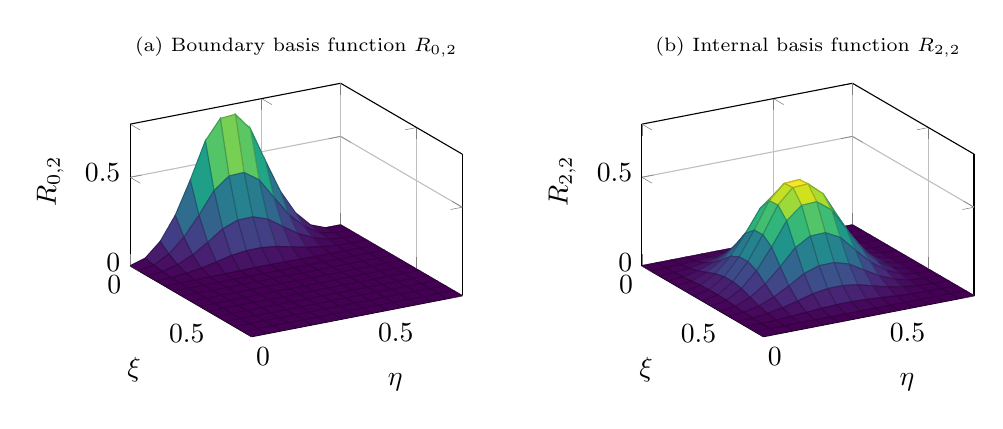
\begin{tikzpicture}[
            declare function={
                n0(\t) = (\t < 0.25) * ((1-4*\t)^2);
                n2(\t) = (\t < 0.25) * (8*\t^2) +
                (\t >= 0.25) * (\t < 0.5) * (12*\t - 16*\t^2 - 1.5) +
                (\t >= 0.5) * (\t < 0.75) * (8*(0.75-\t)^2);
              }
          ]
          % Panel (a) Axis
          \begin{axis}[
              at={(0,0)},
              width=5.8cm,
              height=4.8cm,
              grid=major,
              xlabel={$\xi$},
              ylabel={$\eta$},
              zlabel={$R_{0,2}$},
              colormap/viridis,
              view={60}{30},
              zmin=0, zmax=0.8,
              title={\scriptsize (a) Boundary basis function $R_{0,2}$}
            ]
            \addplot3[
              surf,
              domain=0:0.8,
              domain y=0:0.8,
              samples=15,
              shader=faceted
            ] {n0(x)*n2(y)};
          \end{axis}

          % Panel (b) Axis
          \begin{axis}[
              at={(6.5cm,0)},
              width=5.8cm,
              height=4.8cm,
              grid=major,
              xlabel={$\xi$},
              ylabel={$\eta$},
              zlabel={$R_{2,2}$},
              colormap/viridis,
              view={60}{30},
              zmin=0, zmax=0.8,
              title={\scriptsize (b) Internal basis function $R_{2,2}$}
            ]
            \addplot3[
              surf,
              domain=0:0.8,
              domain y=0:0.8,
              samples=15,
              shader=faceted
            ] {n2(x)*n2(y)};
          \end{axis}
        \end{tikzpicture}
      }
      \\[2pt]
      {\scriptsize 3D surface plot of boundary vs. internal bivariate B-spline functions}
    \end{column}
  \end{columns}
\end{frame}


% Slide: Parametric to Physical Domain Mapping
\begin{frame}{Parametric to Physical Domain Mapping}
  \begin{columns}[T]
    \begin{column}{0.48\textwidth}
      \small
      \textbf{Parent to Physical Space Mapping}:
      \begin{itemize}
        \item Maps the parent parametric square $[0,1]^2$ to the physical 2D domain $\Omega$:
              \[
                \vect{x}(\xi, \eta) = \sum_{i} \sum_{j} R_{i,j}^{p,q}(\xi, \eta) \vect{P}_{i,j}
              \]
        \item \textbf{Spatial Coordinate Jacobian} $\mat{J}_{\boldsymbol{\xi}}$:
              \[
                \mat{J}_{\boldsymbol{\xi}}(\xi,\eta) = \begin{bmatrix} \frac{\partial x}{\partial \xi} & \frac{\partial y}{\partial \xi} \\[0.2em] \frac{\partial x}{\partial \eta} & \frac{\partial y}{\partial \eta} \end{bmatrix}
              \]
        \item \textbf{Differential Element}:
              \[
                \mathrm{d}\Omega = \det(\mat{J}_{\boldsymbol{\xi}})\,\mathrm{d}\xi\,\mathrm{d}\eta
              \]
      \end{itemize}
    \end{column}
    \begin{column}{0.48\textwidth}
      \centering
      \scalebox{0.85}{
        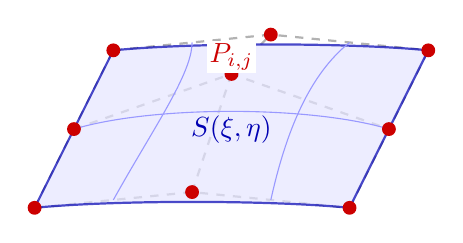
\begin{tikzpicture}[scale=1.0, >=stealth]
          % Row 0 (bottom)
          \coordinate (P00) at (0, 0);
          \coordinate (P10) at (2, 0.2);
          \coordinate (P20) at (4, 0);
          % Row 1 (middle)
          \coordinate (P01) at (0.5, 1.0);
          \coordinate (P11) at (2.5, 1.7); % raised in the middle
          \coordinate (P21) at (4.5, 1.0);
          % Row 2 (top)
          \coordinate (P02) at (1.0, 2.0);
          \coordinate (P12) at (3.0, 2.2);
          \coordinate (P22) at (5.0, 2.0);

          % Draw control net (dashed grid)
          \draw[thick, gray!60, dashed] (P00) -- (P10) -- (P20);
          \draw[thick, gray!60, dashed] (P01) -- (P11) -- (P21);
          \draw[thick, gray!60, dashed] (P02) -- (P12) -- (P22);
          \draw[thick, gray!60, dashed] (P00) -- (P01) -- (P02);
          \draw[thick, gray!60, dashed] (P10) -- (P11) -- (P12);
          \draw[thick, gray!60, dashed] (P20) -- (P21) -- (P22);

          % Draw the smooth surface patch (colored patch)
          \fill[blue!10, opacity=0.7, draw=blue!70!black, thick]
          (P00) .. controls (1.0, 0.1) and (3.0, 0.1) .. (P20)
          .. controls (4.3, 0.6) and (4.7, 1.4) .. (P22)
          .. controls (4.0, 2.1) and (2.0, 2.1) .. (P02)
          .. controls (0.7, 1.4) and (0.3, 0.6) .. (P00);

          % Draw grid lines on the surface patch to show parameter lines
          \draw[blue!40, thin] (1.0, 0.1) .. controls (1.5, 1.0) and (2.0, 1.7) .. (2.0, 2.1);
          \draw[blue!40, thin] (3.0, 0.1) .. controls (3.2, 1.0) and (3.5, 1.7) .. (4.0, 2.1);
          \draw[blue!40, thin] (0.5, 1.0) .. controls (1.5, 1.3) and (3.5, 1.3) .. (4.5, 1.0);

          % Draw control points
          \foreach \p in {P00, P01, P02, P10, P11, P12, P20, P21, P22} {
              \fill[red!80!black] (\p) circle (2.5pt);
            }

          \node[red!80!black, above, fill=white, inner sep=1pt] at (P11) {$\vect{P}_{i,j}$};
          \node[blue!70!black] at (2.5, 1.0) {$\vect{S}(\xi,\eta)$};
        \end{tikzpicture}
      }
      \\[4pt]
      {\scriptsize 2D B-spline surface patch mapping concept}\\[0.15cm]
      \href{https://cnam-internship-mumen.netlify.app/app/simulations/iga-sim-2.1/}{\beamergotobutton{Open 2D Surface Web App}}
    \end{column}
  \end{columns}
\end{frame}

% Slide: h-Refinement (Knot Insertion)
\begin{frame}{$h$-Refinement (Knot Insertion)}
  \begin{columns}[T]
    \begin{column}{0.48\textwidth}
      \small
      \textbf{Knot Insertion}: Adding elements by subdividing knot spans.
      \par\vspace{0.1cm}
      \begin{itemize}
        \item \textbf{Why}: Localize refinement near high-stress areas (e.g., notches).
        \item \textbf{How}: Boehm's algorithm inserts new values $\bar{\xi}$ into $\Xi$.
        \item \textbf{Pros}: Geometry is preserved exactly. Continuity is maintained ($C^{p-1}$).
        \item \textbf{Cons}: Increases mesh size (number of elements) $\to$ larger system matrix $\to$ slower solver.
      \end{itemize}
      \par\vspace{0.2cm}
      \centering
      \href{https://cnam-internship-mumen.netlify.app/app/simulations/iga-sim-1.3/}{\beamerbutton{Interactive $h$-Refinement App}}
    \end{column}
    \begin{column}{0.50\textwidth}
      \centering
      \scalebox{0.72}{
        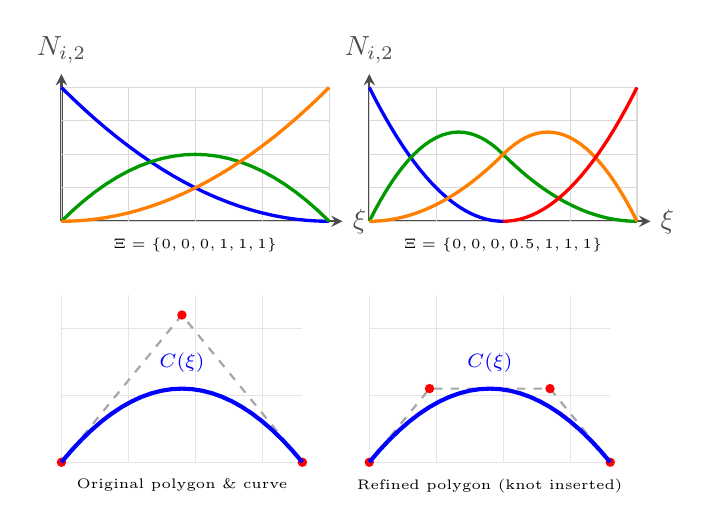
\begin{tikzpicture}[scale=0.85, >=stealth]
          % Row 1: Basis functions before/after
          \begin{scope}[yshift=3.6cm]
            \draw[->, thick, black!70] (0,0) -- (4.2,0) node[right] {$\xi$};
            \draw[->, thick, black!70] (0,0) -- (0,2.2) node[above] {$N_{i,2}$};
            \draw[gray!30, thin] (0,0) grid[ystep=0.5, xstep=1.0] (4,2);
            \draw[blue, line width=1.2pt, domain=0:4] plot (\x, {2*(1 - \x/4)^2});
            \draw[green!60!black, line width=1.2pt, domain=0:4] plot (\x, {2*2*(\x/4)*(1 - \x/4)});
            \draw[orange, line width=1.2pt, domain=0:4] plot (\x, {2*(\x/4)^2});
            \node[font=\tiny, below] at (2, -0.1) {$\Xi = \{0,0,0,1,1,1\}$};
          \end{scope}
          \begin{scope}[xshift=4.6cm, yshift=3.6cm]
            \draw[->, thick, black!70] (0,0) -- (4.2,0) node[right] {$\xi$};
            \draw[->, thick, black!70] (0,0) -- (0,2.2) node[above] {$N_{i,2}$};
            \draw[gray!30, thin] (0,0) grid[ystep=0.5, xstep=1.0] (4,2);
            \draw[blue, line width=1.2pt, domain=0:2] plot (\x, {2*(1 - \x/2)^2});
            \draw[green!60!black, line width=1.2pt, domain=0:2] plot (\x, {2*(4*(\x/4) - 6*(\x/4)^2)});
            \draw[green!60!black, line width=1.2pt, domain=2:4] plot (\x, {2*(2*(1-\x/4)^2)});
            \draw[orange, line width=1.2pt, domain=0:2] plot (\x, {2*(2*(\x/4)^2)});
            \draw[orange, line width=1.2pt, domain=2:4] plot (\x, {2*(4*(1-\x/4) - 6*(1-\x/4)^2)});
            \draw[red, line width=1.2pt, domain=2:4] plot (\x, {2*((\x-2)/2)^2});
            \node[font=\tiny, below] at (2, -0.1) {$\Xi = \{0,0,0,0.5,1,1,1\}$};
          \end{scope}

          % Row 2: Curves and control polygons before/after
          \begin{scope}[xshift=0cm, yshift=0cm]
            \draw[gray!20, thin] (0,0) grid (3.6,2.5);
            \draw[gray!70, dashed, line width=0.8pt] (0,0) -- (1.8,2.2) -- (3.6,0);
            \fill[red] (0,0) circle (2pt);
            \fill[red] (1.8,2.2) circle (2pt);
            \fill[red] (3.6,0) circle (2pt);
            \draw[blue, line width=1.5pt, domain=0:1] plot ({3.6*\x}, {4.4*\x*(1-\x)});
            \node[blue, above, font=\scriptsize] at (1.8, 1.2) {$\vect{C}(\xi)$};
            \node[font=\tiny, below] at (1.8, -0.1) {Original polygon \& curve};
          \end{scope}
          \begin{scope}[xshift=4.6cm, yshift=0cm]
            \draw[gray!20, thin] (0,0) grid (3.6,2.5);
            \draw[gray!70, dashed, line width=0.8pt] (0,0) -- (0.9,1.1) -- (2.7,1.1) -- (3.6,0);
            \fill[red] (0,0) circle (2pt);
            \fill[red] (0.9,1.1) circle (2pt);
            \fill[red] (2.7,1.1) circle (2pt);
            \fill[red] (3.6,0) circle (2pt);
            \draw[blue, line width=1.5pt, domain=0:1] plot ({3.6*\x}, {4.4*\x*(1-\x)});
            \node[blue, above, font=\scriptsize] at (1.8, 1.2) {$\vect{C}(\xi)$};
            \node[font=\tiny, below] at (1.8, -0.1) {Refined polygon (knot inserted)};
          \end{scope}
        \end{tikzpicture}
      }
    \end{column}
  \end{columns}
\end{frame}

% Slide: p-Refinement (Degree Elevation)
\begin{frame}{$p$-Refinement (Degree Elevation)}
  \begin{columns}[T]
    \begin{column}{0.48\textwidth}
      \small
      \textbf{Degree Elevation}: Increasing polynomial degree of basis functions.
      \par\vspace{0.15cm}
      \begin{itemize}
        \item \textbf{Why}: Boost accuracy for smooth solutions and wave dynamics.
        \item \textbf{How}: Linear operator elevates degree $p \to p + \Delta p$, increasing knot multiplicity to preserve continuity.
        \item \textbf{Pros}: Keeps geometric shape identical. Avoids high-order Runge oscillations of Lagrange FEM.
        \item \textbf{Cons}: Wider basis support increases matrix bandwidth and solver overhead.
      \end{itemize}
      \par\vspace{0.2cm}
      \centering
      \href{https://cnam-internship-mumen.netlify.app/app/simulations/iga-sim-1.2/}{\beamerbutton{Interactive $p$-Refinement App}}
    \end{column}
    \begin{column}{0.50\textwidth}
      \centering
      \scalebox{0.72}{
        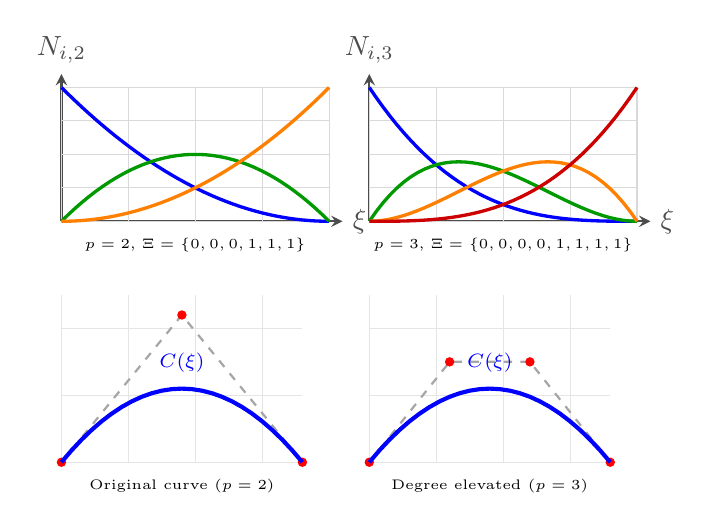
\begin{tikzpicture}[scale=0.85, >=stealth]
          % Row 1: Basis functions before/after (p=2 to p=3)
          \begin{scope}[yshift=3.6cm]
            \draw[->, thick, black!70] (0,0) -- (4.2,0) node[right] {$\xi$};
            \draw[->, thick, black!70] (0,0) -- (0,2.2) node[above] {$N_{i,2}$};
            \draw[gray!30, thin] (0,0) grid[ystep=0.5, xstep=1.0] (4,2);
            \draw[blue, line width=1.2pt, domain=0:4, samples=40] plot (\x, {2*(1 - \x/4)^2});
            \draw[green!60!black, line width=1.2pt, domain=0:4, samples=40] plot (\x, {4*(\x/4)*(1 - \x/4)});
            \draw[orange, line width=1.2pt, domain=0:4, samples=40] plot (\x, {2*(\x/4)^2});
            \node[font=\tiny, below] at (2, -0.1) {$p=2$, $\Xi = \{0,0,0,1,1,1\}$};
          \end{scope}
          \begin{scope}[xshift=4.6cm, yshift=3.6cm]
            \draw[->, thick, black!70] (0,0) -- (4.2,0) node[right] {$\xi$};
            \draw[->, thick, black!70] (0,0) -- (0,2.2) node[above] {$N_{i,3}$};
            \draw[gray!30, thin] (0,0) grid[ystep=0.5, xstep=1.0] (4,2);
            \draw[blue, line width=1.2pt, domain=0:4, samples=40] plot (\x, {2*(1 - \x/4)^3});
            \draw[green!60!black, line width=1.2pt, domain=0:4, samples=40] plot (\x, {6*(\x/4)*(1 - \x/4)^2});
            \draw[orange, line width=1.2pt, domain=0:4, samples=40] plot (\x, {6*(\x/4)^2*(1 - \x/4)});
            \draw[red!80!black, line width=1.2pt, domain=0:4, samples=40] plot (\x, {2*(\x/4)^3});
            \node[font=\tiny, below] at (2, -0.1) {$p=3$, $\Xi = \{0,0,0,0,1,1,1,1\}$};
          \end{scope}

          % Row 2: Curves and control polygons before/after
          \begin{scope}[xshift=0cm, yshift=0cm]
            \draw[gray!20, thin] (0,0) grid (3.6,2.5);
            \draw[gray!70, dashed, line width=0.8pt] (0,0) -- (1.8,2.2) -- (3.6,0);
            \fill[red] (0,0) circle (2pt);
            \fill[red] (1.8,2.2) circle (2pt);
            \fill[red] (3.6,0) circle (2pt);
            \draw[blue, line width=1.5pt, domain=0:1] plot ({3.6*\x}, {4.4*\x*(1-\x)});
            \node[blue, above, font=\scriptsize] at (1.8, 1.2) {$\vect{C}(\xi)$};
            \node[font=\tiny, below] at (1.8, -0.1) {Original curve ($p=2$)};
          \end{scope}
          \begin{scope}[xshift=4.6cm, yshift=0cm]
            \draw[gray!20, thin] (0,0) grid (3.6,2.5);
            \draw[gray!70, dashed, line width=0.8pt] (0,0) -- (1.2,1.5) -- (2.4,1.5) -- (3.6,0);
            \fill[red] (0,0) circle (2pt);
            \fill[red] (1.2,1.5) circle (2pt);
            \fill[red] (2.4,1.5) circle (2pt);
            \fill[red] (3.6,0) circle (2pt);
            \draw[blue, line width=1.5pt, domain=0:1] plot ({3.6*\x}, {4.4*\x*(1-\x)});
            \node[blue, above, font=\scriptsize] at (1.8, 1.2) {$\vect{C}(\xi)$};
            \node[font=\tiny, below] at (1.8, -0.1) {Degree elevated ($p=3$)};
          \end{scope}
        \end{tikzpicture}
      }
    \end{column}
  \end{columns}
\end{frame}

% Slide: k-Refinement & Exact Geometry
\begin{frame}{$k$-Refinement \& Exact Geometry}
  \begin{columns}[T]
    \begin{column}{0.52\textwidth}
      \small
      \textbf{k-Refinement}: Elevating polynomial degree while maintaining maximum inter-element continuity.
      \par\vspace{0.15cm}
      \begin{itemize}
        \item \textbf{Why}: Achieve maximum accuracy per DOF. High continuity ($C^{p-1}$) is optimal for dynamics.
        \item \textbf{How}: Elevate degree first ($p \to p+\Delta p$), \textit{then} insert internal knots.
        \item \textbf{Pros}: Unique to IGA. Keeps DOFs minimal for a given error tolerance.
        \item \textbf{Cons}: Higher computational assembly stencil (wider support).
      \end{itemize}
      \par\vspace{0.2cm}
      \centering
      \href{https://cnam-internship-mumen.netlify.app/app/simulations/iga-sim-1.5/}{\beamerbutton{Interactive $k$-Refinement App}}
    \end{column}
    \begin{column}{0.45\textwidth}
      \begin{alertblock}{Continuity Comparison}
        \centering\scriptsize
        \begin{tabular}{lcc}
          \toprule
          \textbf{Method}  & \textbf{Sequence}      & \textbf{Continuity}           \\
          \midrule
          $h \to p$        & Insert first           & $C^0$ (FEA-like)              \\
          \textbf{$k$-ref} & \textbf{Elevate first} & \textbf{$C^{p+\Delta p - 1}$} \\
          \bottomrule
        \end{tabular}
      \end{alertblock}
      \vspace{0.05cm}
      \centering
      \scalebox{0.68}{
        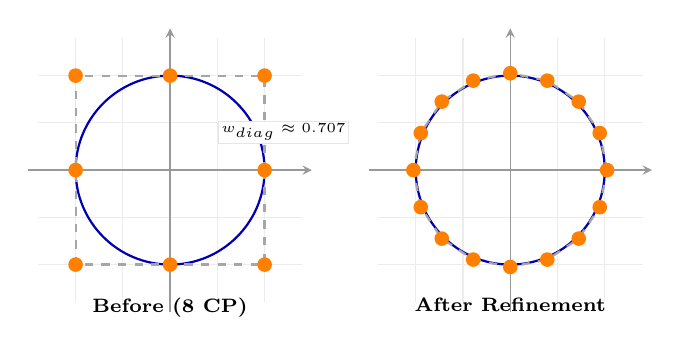
\begin{tikzpicture}[scale=1.2, >=stealth]
          % --- PANEL (a) BEFORE ---
          \begin{scope}[xshift=0cm]
            \draw[gray!15, thin, step=0.5] (-1.4, -1.4) grid (1.4, 1.4);
            \draw[->, black!40, line width=0.5pt] (-1.5, 0) -- (1.5, 0);
            \draw[->, black!40, line width=0.5pt] (0, -1.5) -- (0, 1.5);
            \draw[blue!70!black, thick] (0,0) circle (1.0);
            \draw[gray!70, dashed, thick] (1,0) -- (1,1) -- (0,1) -- (-1,1) -- (-1,0) -- (-1,-1) -- (0,-1) -- (1,-1) -- cycle;
            \foreach \x/\y in {1/0, 0/1, -1/0, 0/-1, 1/1, -1/1, -1/-1, 1/-1} {
                \fill[orange] (\x, \y) circle (2.2pt);
              }
            \node[font=\tiny, fill=white, inner sep=1pt, draw=gray!20] at (1.2, 0.4) {$w_{\text{diag}}\approx 0.707$};
            \node[below=1.5cm, font=\scriptsize\bfseries] at (0,0) {Before (8 CP)};
          \end{scope}

          % --- PANEL (b) AFTER ---
          \begin{scope}[xshift=3.6cm]
            \draw[gray!15, thin, step=0.5] (-1.4, -1.4) grid (1.4, 1.4);
            \draw[->, black!40, line width=0.5pt] (-1.5, 0) -- (1.5, 0);
            \draw[->, black!40, line width=0.5pt] (0, -1.5) -- (0, 1.5);
            \draw[blue!70!black, thick] (0,0) circle (1.0);
            \draw[gray!70, dashed, thick] (0:1.025)
            \foreach \angle in {22.5, 45, 67.5, 90, 112.5, 135, 157.5, 180, 202.5, 225, 247.5, 270, 292.5, 315, 337.5, 360} {
                -- (\angle:1.025)
              };
            \foreach \angle in {0, 22.5, 45, 67.5, 90, 112.5, 135, 157.5, 180, 202.5, 225, 247.5, 270, 292.5, 315, 337.5} {
                \fill[orange] (\angle:1.025) circle (2.2pt);
              }
            \node[below=1.5cm, font=\scriptsize\bfseries] at (0,0) {After Refinement};
          \end{scope}
        \end{tikzpicture}
      }
      \par\vspace{0.05cm}
      {\tiny Exact circle: diagonal weights $w_i = \frac{\sqrt{2}}{2}$. Knot insertion converges net to curve.}
    \end{column}
  \end{columns}
\end{frame}

% Slide: Isoparametric Concept & Field Approximation
\begin{frame}{Isoparametric Concept \& Field Approximation}
  \begin{columns}[T]
    \begin{column}{0.48\textwidth}
      \small
      \textbf{The Isoparametric Paradigm}:
      The \textbf{same NURBS basis} $R_a$ represents geometry and field variables:
      \[
        \underbrace{\vect{x}(\xi) = \sum_a R_a\,\vect{P}_a}_{\text{\scriptsize Geometry}}, \quad
        \underbrace{\vect{u}^h(\xi, t) = \sum_a R_a\,\vect{u}_a(t)}_{\text{\scriptsize Displacement}}
      \]
      \vspace{-0.25cm}
      \begin{itemize}
        \footnotesize
        \setlength{\itemsep}{0.1cm}
        \item \textbf{Control Displacements $\vect{u}_a(t)$}: Displacing $\vect{P}_a \to \vect{P}_a + \vect{u}_a$ smoothly deforms the continuum.
        \item \textbf{Inherited Regularity}: $\vect{u}^h \in C^{p-1} \implies$ continuous strain and stress fields across elements.
        \item \textbf{Discrete State}: $\vect{U}(t) \in \mathbb{R}^{2N_{\text{cp}}}$ directly enters the dynamic FOM in Chapter~4.
      \end{itemize}
    \end{column}

    \begin{column}{0.50\textwidth}
      \centering
      \scalebox{0.70}{
        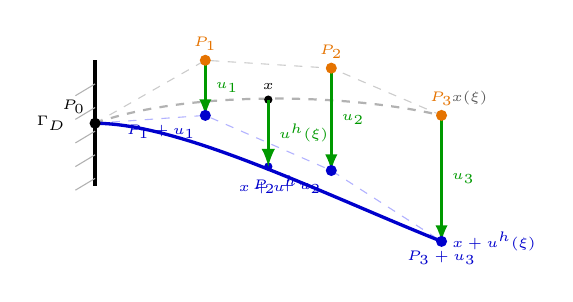
\begin{tikzpicture}[scale=1.0, >=stealth]
          % Wall (clamped boundary)
          \draw[line width=1.2pt] (0,2.1) -- (0,0.5);
          \foreach \y in {0.6,0.9,...,2.0} {
            \draw[gray!60] (0,\y) -- (-0.25,\y-0.15);
          }
          \node[left, font=\tiny] at (-0.25, 1.3) {$\Gamma_D$};

          % Coordinates
          \coordinate (P0) at (0, 1.3);
          \coordinate (P1) at (1.4, 2.1);
          \coordinate (P2) at (3.0, 2.0);
          \coordinate (P3) at (4.4, 1.4);

          \coordinate (P1d) at (1.4, 1.4);
          \coordinate (P2d) at (3.0, 0.7);
          \coordinate (P3d) at (4.4, -0.2);

          % Original control net
          \draw[gray!40, dashed, thin] (P0) -- (P1) -- (P2) -- (P3);
          % Deformed control net
          \draw[blue!30, dashed, thin] (P0) -- (P1d) -- (P2d) -- (P3d);

          % Original curve
          \draw[thick, gray!60, dashed] (P0) .. controls (1.1, 1.7) and (3.1, 1.7) .. (P3)
            node[above right, font=\tiny, gray!70!black] {$\vect{x}(\xi)$};

          % Deformed curve
          \draw[very thick, blue!80!black] (P0) .. controls (1.1, 1.3) and (2.9, 0.4) .. (P3d)
            node[right, font=\tiny, blue!80!black] {$\vect{x} + \vect{u}^h(\xi)$};

          % Displacement vectors at control points
          \draw[->, >=latex, line width=1.0pt, green!60!black] (P1) -- (P1d)
            node[midway, right, font=\tiny] {$\vect{u}_1$};
          \draw[->, >=latex, line width=1.0pt, green!60!black] (P2) -- (P2d)
            node[midway, right, font=\tiny] {$\vect{u}_2$};
          \draw[->, >=latex, line width=1.0pt, green!60!black] (P3) -- (P3d)
            node[midway, right, font=\tiny] {$\vect{u}_3$};

          % Physical point displacement
          \coordinate (X) at (2.2, 1.6);
          \coordinate (Xd) at (2.2, 0.75);
          \fill[black] (X) circle (1.5pt) node[above, font=\tiny] {$\vect{x}$};
          \fill[blue!80!black] (Xd) circle (1.5pt) node[below, font=\tiny] {$\vect{x}+\vect{u}^h$};
          \draw[->, >=latex, line width=1.2pt, green!60!black] (X) -- (Xd)
            node[midway, right, font=\tiny\bfseries] {$\vect{u}^h(\xi)$};

          % Control points
          \fill[orange!90!black] (P1) circle (2pt) node[above, font=\tiny] {$\vect{P}_1$};
          \fill[orange!90!black] (P2) circle (2pt) node[above, font=\tiny] {$\vect{P}_2$};
          \fill[orange!90!black] (P3) circle (2pt) node[above, font=\tiny] {$\vect{P}_3$};

          \fill[blue!80!black] (P1d) circle (2pt) node[below left, font=\tiny] {$\vect{P}_1+\vect{u}_1$};
          \fill[blue!80!black] (P2d) circle (2pt) node[below left, font=\tiny] {$\vect{P}_2+\vect{u}_2$};
          \fill[blue!80!black] (P3d) circle (2pt) node[below, font=\tiny] {$\vect{P}_3+\vect{u}_3$};

          \fill[black] (P0) circle (2pt) node[above left, font=\tiny] {$\vect{P}_0$};
        \end{tikzpicture}
      }
      \par\vspace{0.05cm}
      {\scriptsize
        \tikz{\fill[orange!90!black] (0,0) circle (2pt);} $\vect{P}_a$ \quad
        \tikz{\fill[blue!80!black] (0,0) circle (2pt);} $\vect{P}_a+\vect{u}_a$ \quad
        \tikz{\draw[->, >=latex, green!60!black, thick] (0,0) -- (0.3,0);} $\vect{u}_a, \vect{u}^h$ \quad
        \tikz{\draw[very thick, blue!80!black] (0,0) -- (0.35,0);} Deformed
      }
    \end{column}
  \end{columns}
\end{frame}

